\documentclass{article}
\usepackage{amsmath}
\usepackage{graphicx}
\begin{document}
\title{Coordinate Geometry Unit Exam: Question 24}
\author{Ana Bhattacharjee}
\date{\today}
\maketitle{}

\begin{center}
The given image required to solve the problem is shown below.
\begin{figure}[!htbp]
  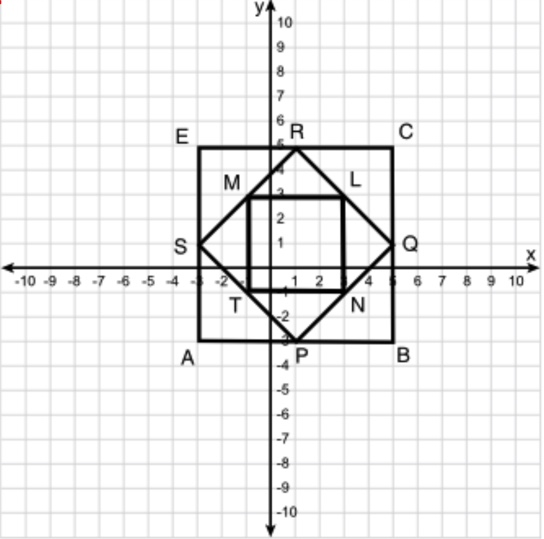
\includegraphics[width=0.9\columnwidth]{q24_figure}
  \caption{Graphic}
\end{figure}
\par
The information given to us is the following:
\begin{itemize}
  \item Points S, P, Q, and R are midpoints of ABCE
  \item T, N, L, and M are midpoints of PQRS
\end{itemize}
\newpage
Since this problem involves the use of midpoints, distances, and slopes, let's first get the coordinates of the points that we need to use to find ML's equation. We first need to find the endpoints of the segment where M is which happens to be R and S. R and S are both midpoints for separate segments, EC and AE respectively. Therefore, the problem starts by knowing the coordinates of E, C, and A.
\begin{align}
  E = 
\end{align}
\end{center}
\end{document}
